%%---------------Laboratorijas darbi-P02, P03, LaTeX, Viljams Vidauskis, REBMO2
\documentclass[a4paper,10pt]{report}
\usepackage[utf8]{inputenc}
%%\usepackage{polyglossia}
\usepackage{graphicx}
\usepackage{epstopdf}
\usepackage{siunitx} %% simboliem, oma utt.
\usepackage{float}
\usepackage{biblatex}
\usepackage[siunitx ,europeanresistors ,americaninductors]{circuitikz} %%elektr.shemam.
\usepackage{tikz} %%elektr.shemam
\usepackage{pgfplots} %%funkciju zimesanai
\pgfplotsset{compat=1.15} %%savietojamībai
\usepackage{amsmath} %%matematisko f attelosanai
%%\DeclareGraphicsExtensions{.ps}
\title{1. laboratorijas darba ”Vienkāršu elektrisku shēmu modelēšana” atskaite}
\author{Viljams Vidauskis}
\begin{document}
\maketitle
\chapter{Teorētiskā daļa}
\section{Ķēdes aprēķins}
Apēķiniet spriegumus uz rezistoriem 1. attēlā dotajā shēmā. Sprieguma avota V1 sprieguma
vērtību U (Voltos) izvēlieties daļskaitli, kas būtu Jūsu apliecības pēdējie trīs cipari dalīti ar
10. Piemēram. ‘101REB123’ nozīmē V1 = 12.3 (Volti), R1 ir apliecības pēdējo 3 ciparu otrais
numurs+1, R2 ir apliecības numura pēdējais cipars +1. Piemēram, ja Jūsu apliecības numurs
ir ‘101REB123’ tad ‘R1=3’, ‘R2=4’. Nofotografējiet aprēķinu vai saglabājiet lapiņu. Aprēķina gaita
būs nepieciešama darbā ‘P02’. Turklāt, aprēķins būs jāpievieno atskaitei, ko veiksiet semestra
beigās.
Mans studenta apl.nr.=171REB174, aprēķinot iegūstu sekojošas
\begin{table}[h]
\centering
\caption{Ķēdes komponenšu vērtības:}
%%\label{my-label}
\begin{tabular}{|l|l|}
\hline
R1  & 8\SI{1}{\ohm} \\ \hline
R2  & 5\SI{1}{\ohm} \\ \hline
V1  &  17.4V \\ \hline
Ur2 &  6.69V \\ \hline
Ur1 &  10.71V \\ \hline
\end{tabular}
\end{table}

UR1 un UR2 vērtības tika aprēķinātas, izmantojot sprieguma dalītāja formulu.
\begin{equation} 
\begin{split}
Ur_2 = V_1* \frac{R_2}{R_1+R_2}
 \end{split}
\end{equation}

\begin{figure}[H]
  \begin{center}
    \begin{circuitikz}
      \draw (0,0)
      to[V,v=$V1 17.4V$] (0,2)
      to[R=$R_1\SI{8}{\ohm}$] (2,2)
      to[R=$R_2\SI{5}{\ohm}$] (2,0)
      to[short] (0,0);
    \end{circuitikz}
    \caption{Uzdevuma principiālā shēma, veidota ar "circuitikz".}
  \end{center}
\end{figure}


Teorētiskā $U_R{}_2$ atkarība no $R_2$
\begin{figure}[H]
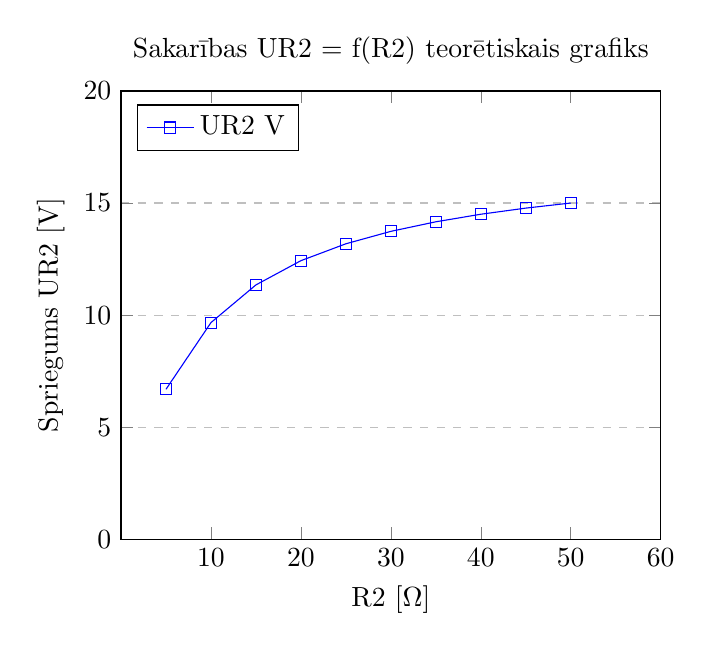
\begin{tikzpicture}
\begin{axis}[
    title={Sakarības UR2 = f(R2) teorētiskais grafiks},
    xlabel={R2 [\SI{}{\ohm}]},
    ylabel={Spriegums UR2 [V]},
    xmin=0, xmax=60,
    ymin=0, ymax=20,
    xtick={10,20,30,40,50,60},
    ytick={0,5,10,15,20},
    legend pos=north west,
    ymajorgrids=true,
    grid style=dashed,
]

\addplot[
    color=blue,
    mark=square,
    ]
    coordinates {
    (5,{(17.4)*((5)/(5+8))})(10,{(17.4)*((10)/(10+8))})(15,{(17.4)*((15)/(15+8))})(20,{(17.4)*((20)/(20+8))})(25,{(17.4)*((25)/(25+8))})(30,{(17.4)*((30)/(30+8))})(35,{(17.4)*((35)/(35+8))})(40,{(17.4)*((40)/(40+8))})(45,{(17.4)*((45)/(45+8))})(50,{(17.4)*((50)/(50+8))})
    };
    \legend{UR2 V}
 
\end{axis}
\end{tikzpicture}
\end{figure}
\chapter{Praktiskā daļa}
\section{Darbs ar GEDA programmām}
\subsection{darbs ar gschem}
\begin{figure}[h]
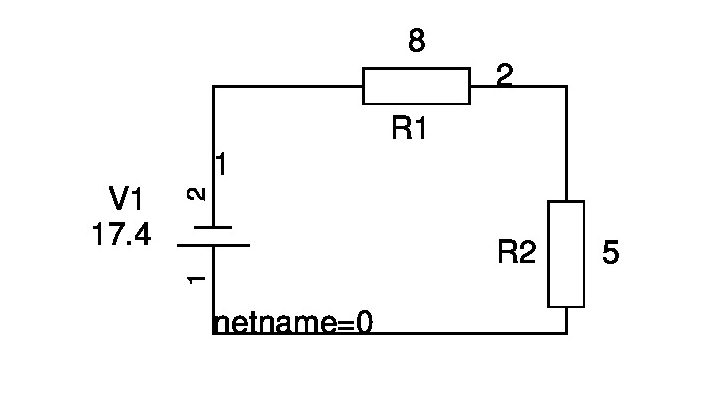
\includegraphics{01.jpg}
\caption{attēls, ir dota elektriskā shēma}
%%\label{}
\end{figure}
\subsection{darbs ar gnetlist}
\begin{verbatim}
* Spice netlister for gnetlist
V1 0 1 17.4
R2 0 2 5
R1 1 2 8
.END
\end{verbatim}
\subsection{darbs ar ngspice}
\begin{figure}[H]
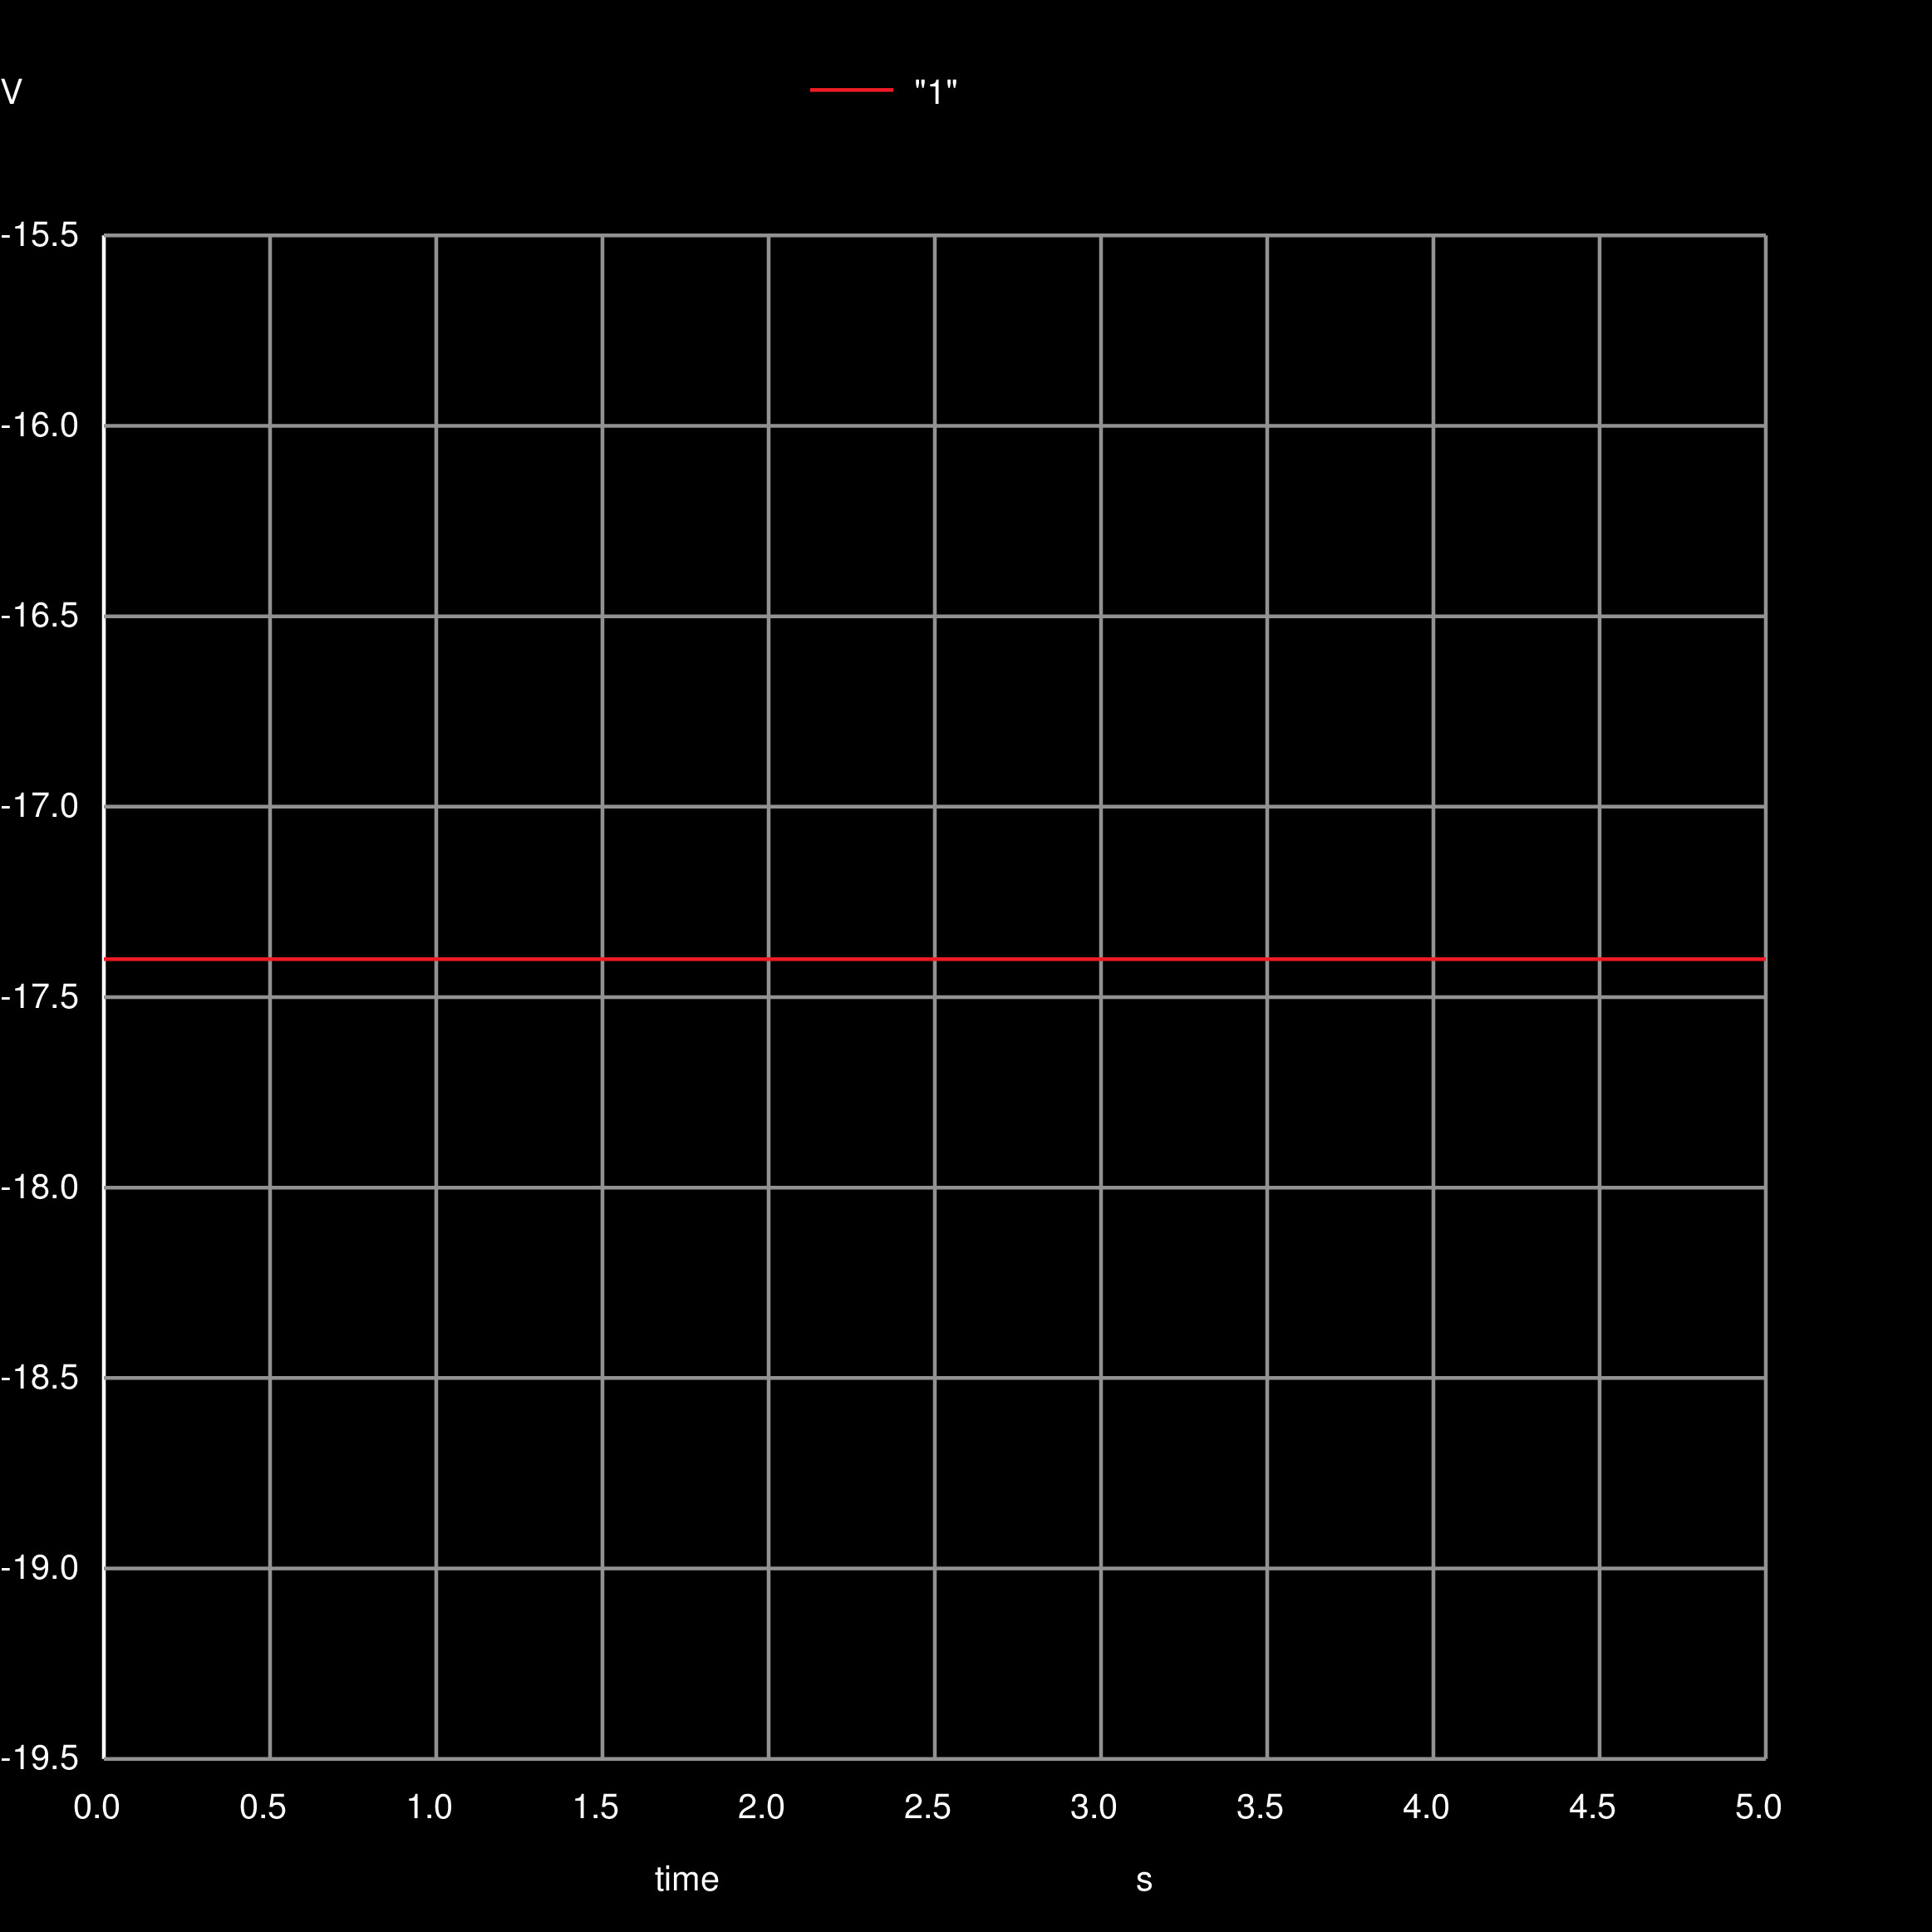
\includegraphics[width=8cm,height=8cm,keepaspectratio]{011.jpg}
\caption{attēls, Spriegums uz rezistora R1}
%%\label{}
\end{figure}
\begin{figure}[H]
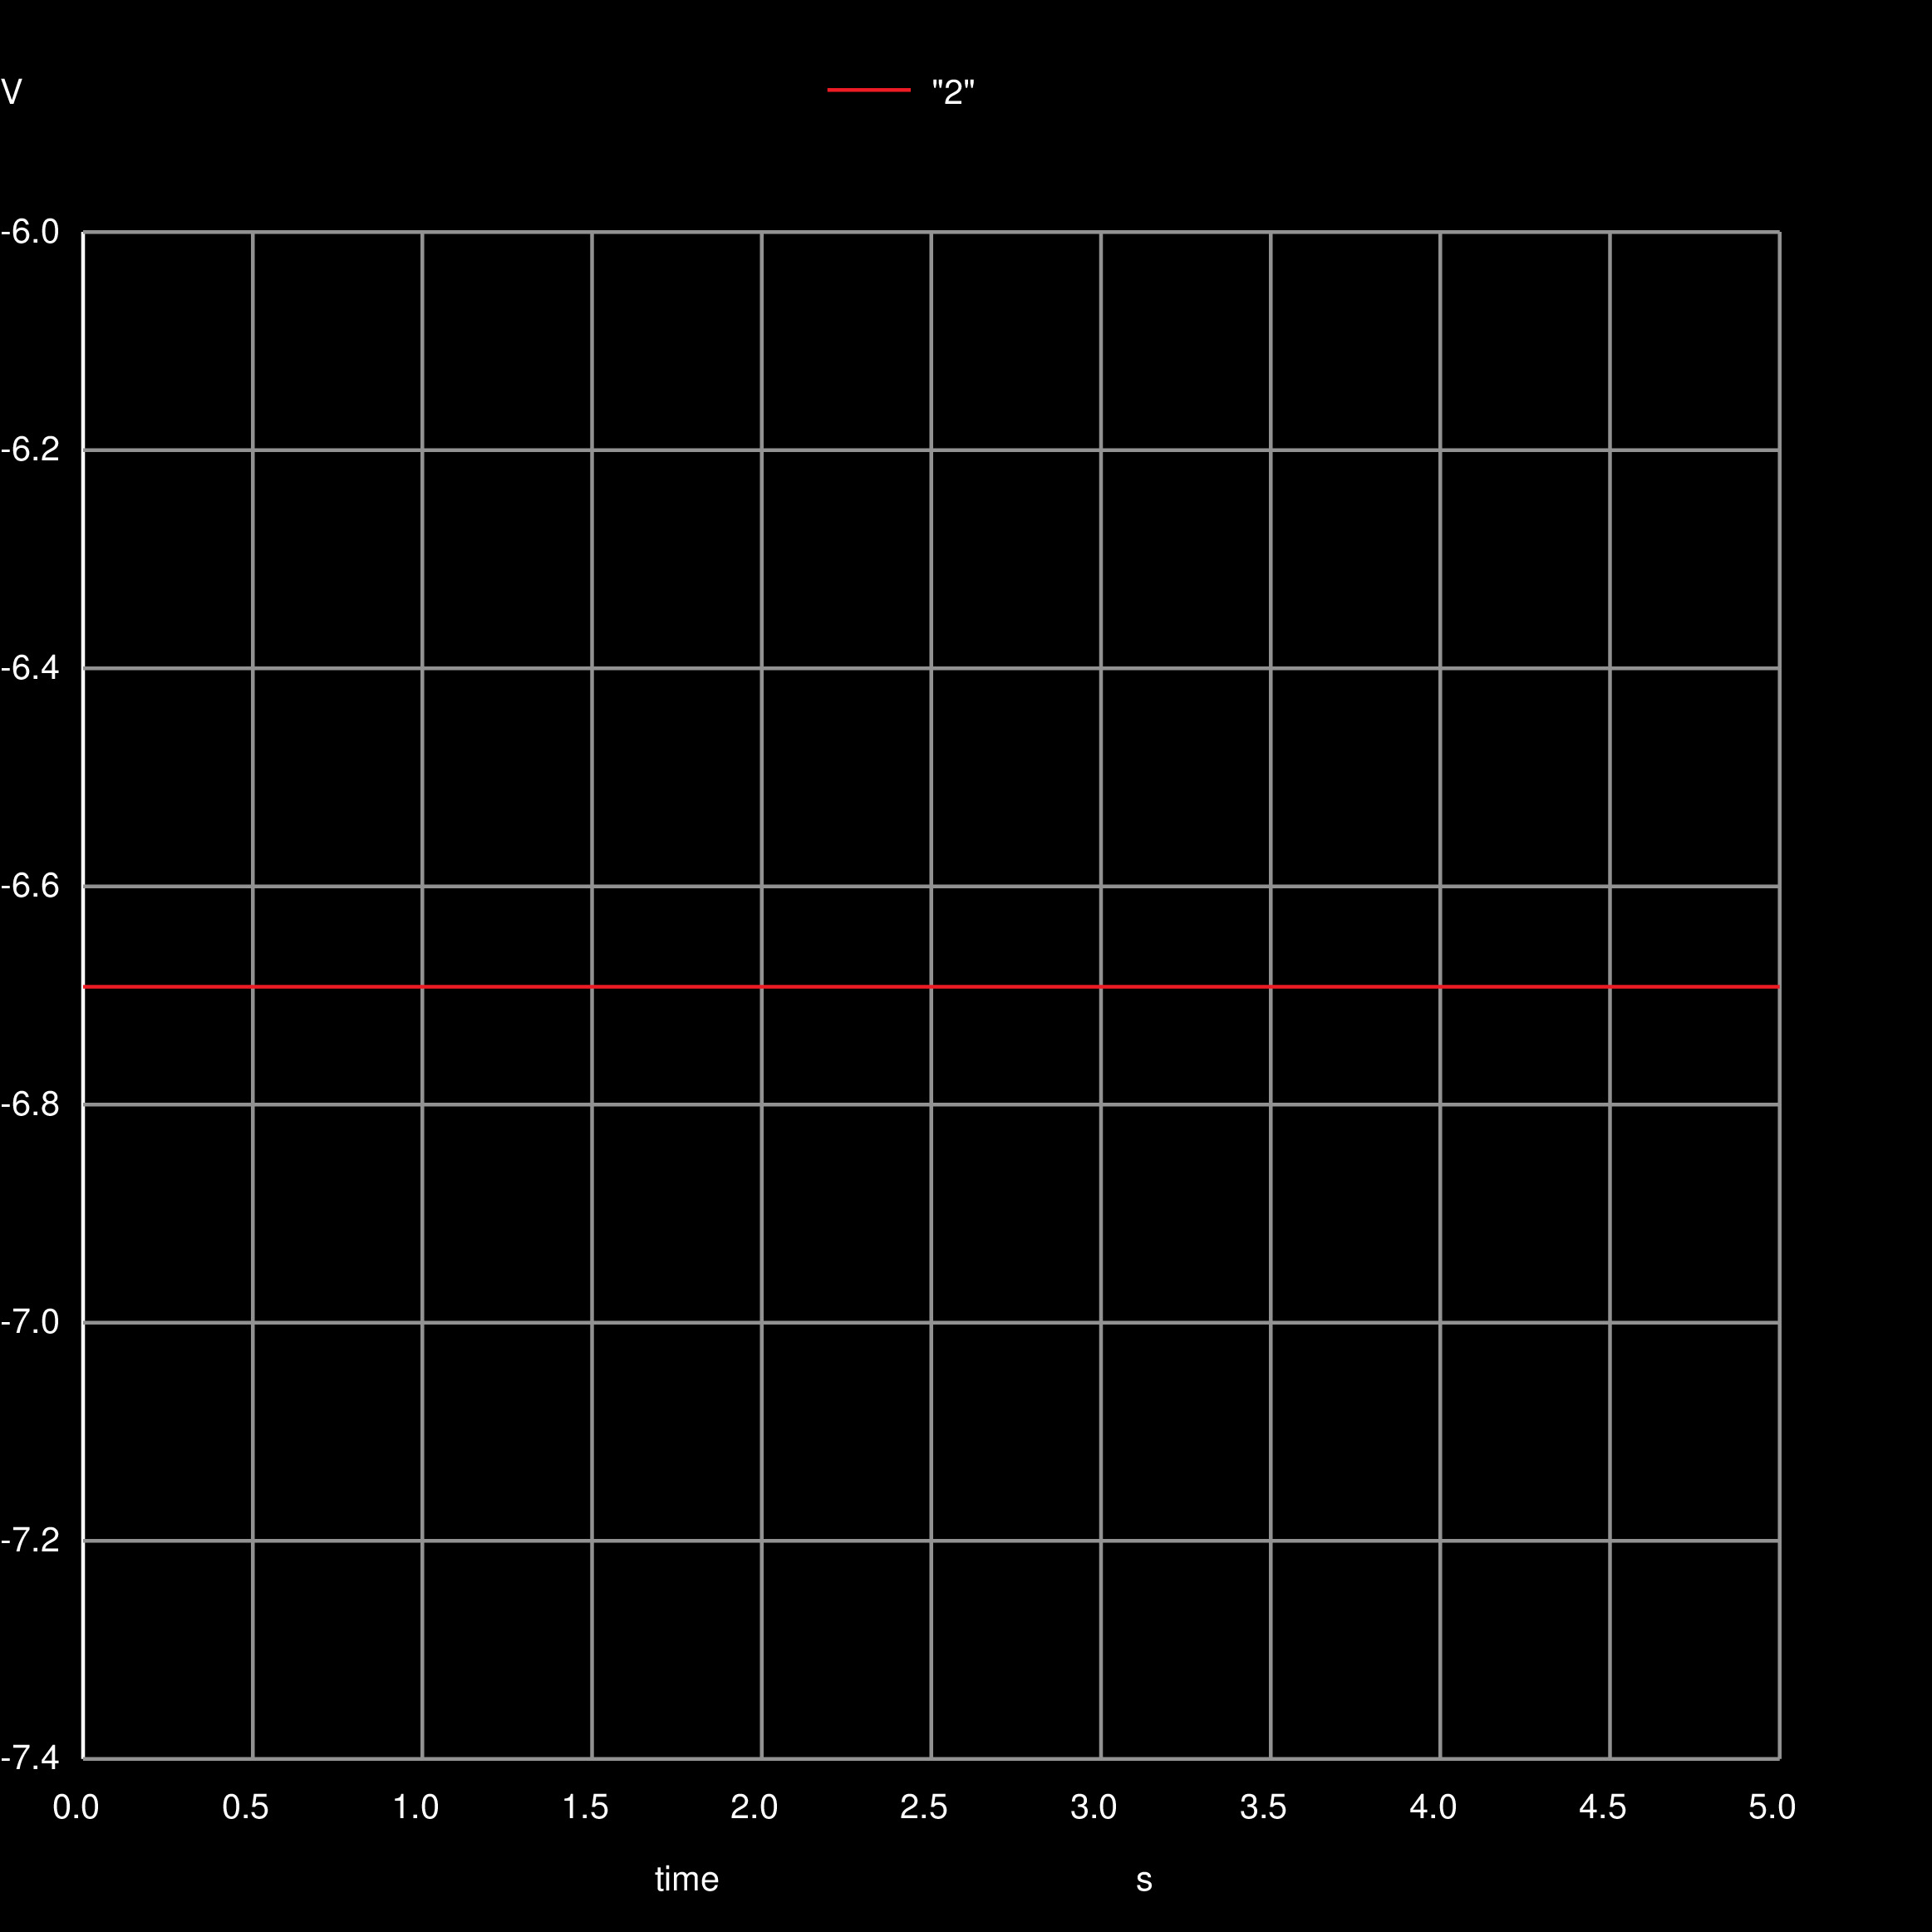
\includegraphics[width=8cm,height=8cm,keepaspectratio]{022.jpg}
\caption{attēls, Spriegums uz rezistora R2}
%%\label{}
\end{figure}
\section{Darbs ar QUCS programmām}
Linux vidē izmantojot QUCS (Quite Universal Circuit Simulator),
tika uzzimēta attēlā redzamā shēma:

\begin{figure}[H]
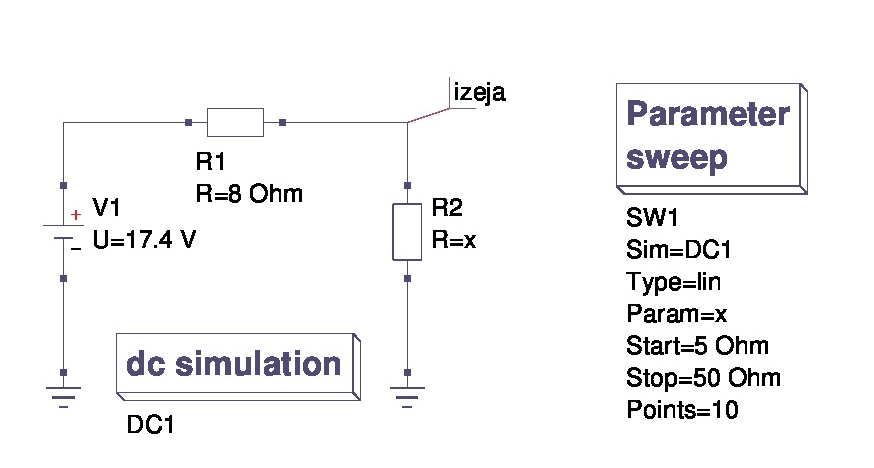
\includegraphics{qucsShema.jpg}
\caption{attēls, QUCS shēma}
%%\label{}
\end{figure}
Iesakumā tika veikta DC simulācija, pieņemot, ka rezistora R2 vērtība ir nemainīga = 5 Ohm
\begin{figure}[H]
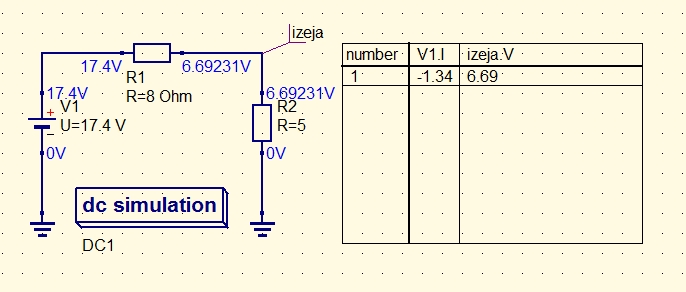
\includegraphics[width=300px,height=200px,keepaspectratio]{qucsDCsim.jpg}
\caption{attēls, QUCS DC simulācija}
%%\label{}
\end{figure}
Shemā esošā rezistora R2 pretestības vērtībai tika piešķirts parametrs x, kuru DC Sweep simulators mainīs robežās no 5 līdz 50 Ohm ar 10 punktiem, jeb soli - 5 Ohm.
Attēlā redzamais grafiks attēlo sakarību starp spriegumu punktā "Izeja" un Rezistora R2 vērtību (x).

\begin{figure}[H]
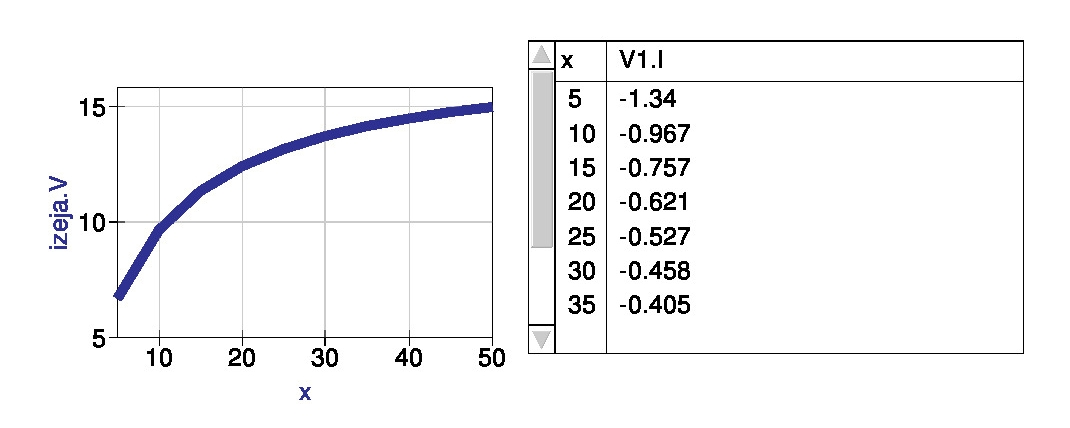
\includegraphics[width=300px,height=120px,keepaspectratio]{qucsSimulacija.jpg}
\caption{attēls, QUCS DC sweep simulācija, Sprieguma UR2 atkarība no pretestības R2}
%%\label{}
\end{figure}
Tabulā ir attēlots x parametra vērtība Omos un caur "Izeja" plūstošās strāvas stiprums.

\begin{thebibliography}{2}
\bibitem{latex1} 
Learn \LaTeX\ online:
\texttt{https://www.sharelatex.com/learn}

\bibitem{qucs1} 
\textit{QUCS FAQ WWW}
\texttt{http://qucs.sourceforge.net/faq.html} 
QUCS Frequently asked Questions
\end{thebibliography}
\end{document}
